
\begin{figure}[h]
	\centering

	\begin{tabularx}{\textwidth}{ p{.2\textwidth} | p{.2\textwidth} | X }
		\textbf{Akteur} & \textbf{Beschreibung} & \textbf{Verwendet in Anwendungsszenario} \\ \hline
		Administrator & Kann Dienste erstellen, andere Nutzer zu Administratoren ernennen und besitzt die gleichen Funktionen wie Website-Nutzer &
			\begin{itemize}
        \item Admin2 - Format erstellen
        \item Admin3 - Dienst erstellen
        \item Admin5 - Administrator ernennen
			\end{itemize} \\ \hline
		Benutzer - Webseite (mit Account) & Kombinationen erstellen, öffnen, speichern und freigeben, Dienst suchen, anzeigen und Account verwalten &
			\begin{itemize}
				\item Acc1 - Accountmanagement
				\item Acc2 - Kombination erstellen
				\item All1 - Dienst suchen
				\item All3 - Kombination suchen
			\end{itemize} \\ \hline
		Benutzer - Webseite (ohne Account) & Dienste und Kombinationen suchen und anzeigen &
			\begin{itemize}
				\item All1 - Dienst suchen
				\item All3 - Kombination suchen
				\item All5 - Registrieren
			\end{itemize} \\ \hline
		Benutzer - App & Kombinationen und Dienste suchen und anzeigen, Kombinationen versenden &
			\begin{itemize}
				\item A1 - Kombination ansehen
        \item A2 - Kombination suchen
        \item A3 - Dienst suchen
			\end{itemize} \\ \hline
	\end{tabularx}

	\caption{Beschreibung der Akteure}
	\label{fig:akteur-tabelle}
\end{figure}


%%%%%%%%%%%%%%%
%% Anwendungsfall 1 %%
%%%%%%%%%%%%%%%
\newpage
\section{Anwendungsfalldiagramm - App}

\begin{figure}[h]
	\centering
	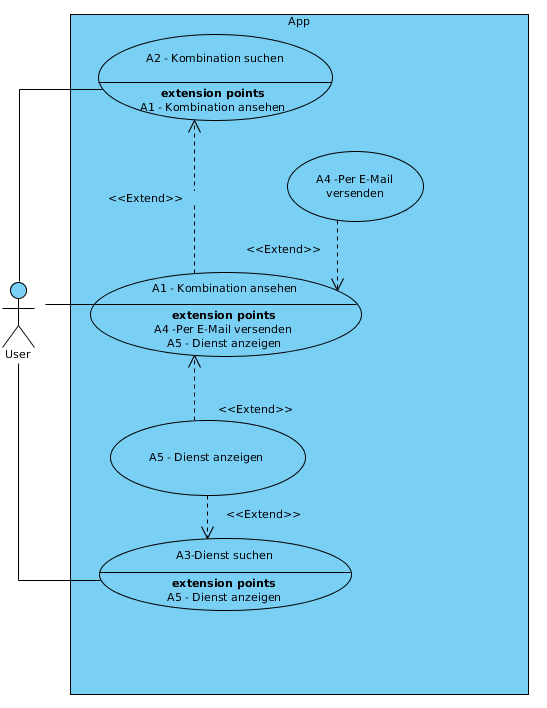
\includegraphics[keepaspectratio,width=11cm]{img/app}
	\caption{Anwendungsfalldiagramm - App}
	\label{fig:anwendungsfalldiagramm-app}
\end{figure}

\newpage

\begin{figure}[h]
	\centering
	\begin{tabularx}{\textwidth}{ X | X }
		\textbf{Anwendungsfall ID} & A4 \\ \hline
		\textbf{Anwendungsfallname} & Per E-Mail versenden \\ \hline
		\textbf{Initiierender Akteur} & Benutzer \\ \hline
		\textbf{Weitere Akteure} & -  \\ \hline
		\textbf{Kurzbeschreibung} & Der Benutzer hat bei der Ansicht einer Kombination die Möglichkeit, diese per E-Mail zu versenden. Dabei wird eine PDF generiert und das Standard E-Mail Programm wird geöffnet.  \\ \hline
		\textbf{Vorbedingungen} & Man hat eine nicht leere Kombination geöffnet.  \\ \hline
		\textbf{Nachbedingungen} & Die Standard E-Mail App wurde geöffnet und enthält das PDF im Anhang.  \\ \hline
		\textbf{Ablauf} &
			\begin{enumerate}
				\item Der Benutzer klickt auf den E-Mail senden Knopf.
        \item Eine PDF Datei wird generiert.
				\item Das Standard E-Mail Programm wird mit der PDF Datei im Anhang geöffnet.
			\end{enumerate} \\ \hline
		\textbf{Alternative} &
			- \\ \hline
		\textbf{Ausnahme} &
			- \\ \hline
		\textbf{Benutzte Anwendungsfälle} & - \\ \hline
	\end{tabularx}
	\caption{Anwendungsfall A4}
	\label{fig:anwendungsfall-app-tabelle-xx-1}
\end{figure}

\newpage


%%%%%%%%%%%%%%%
%% Anwendungsfall 2 %%
%%%%%%%%%%%%%%%

\section{Anwendungsfalldiagramm - Server}

\begin{figure}[h]
	\centering
	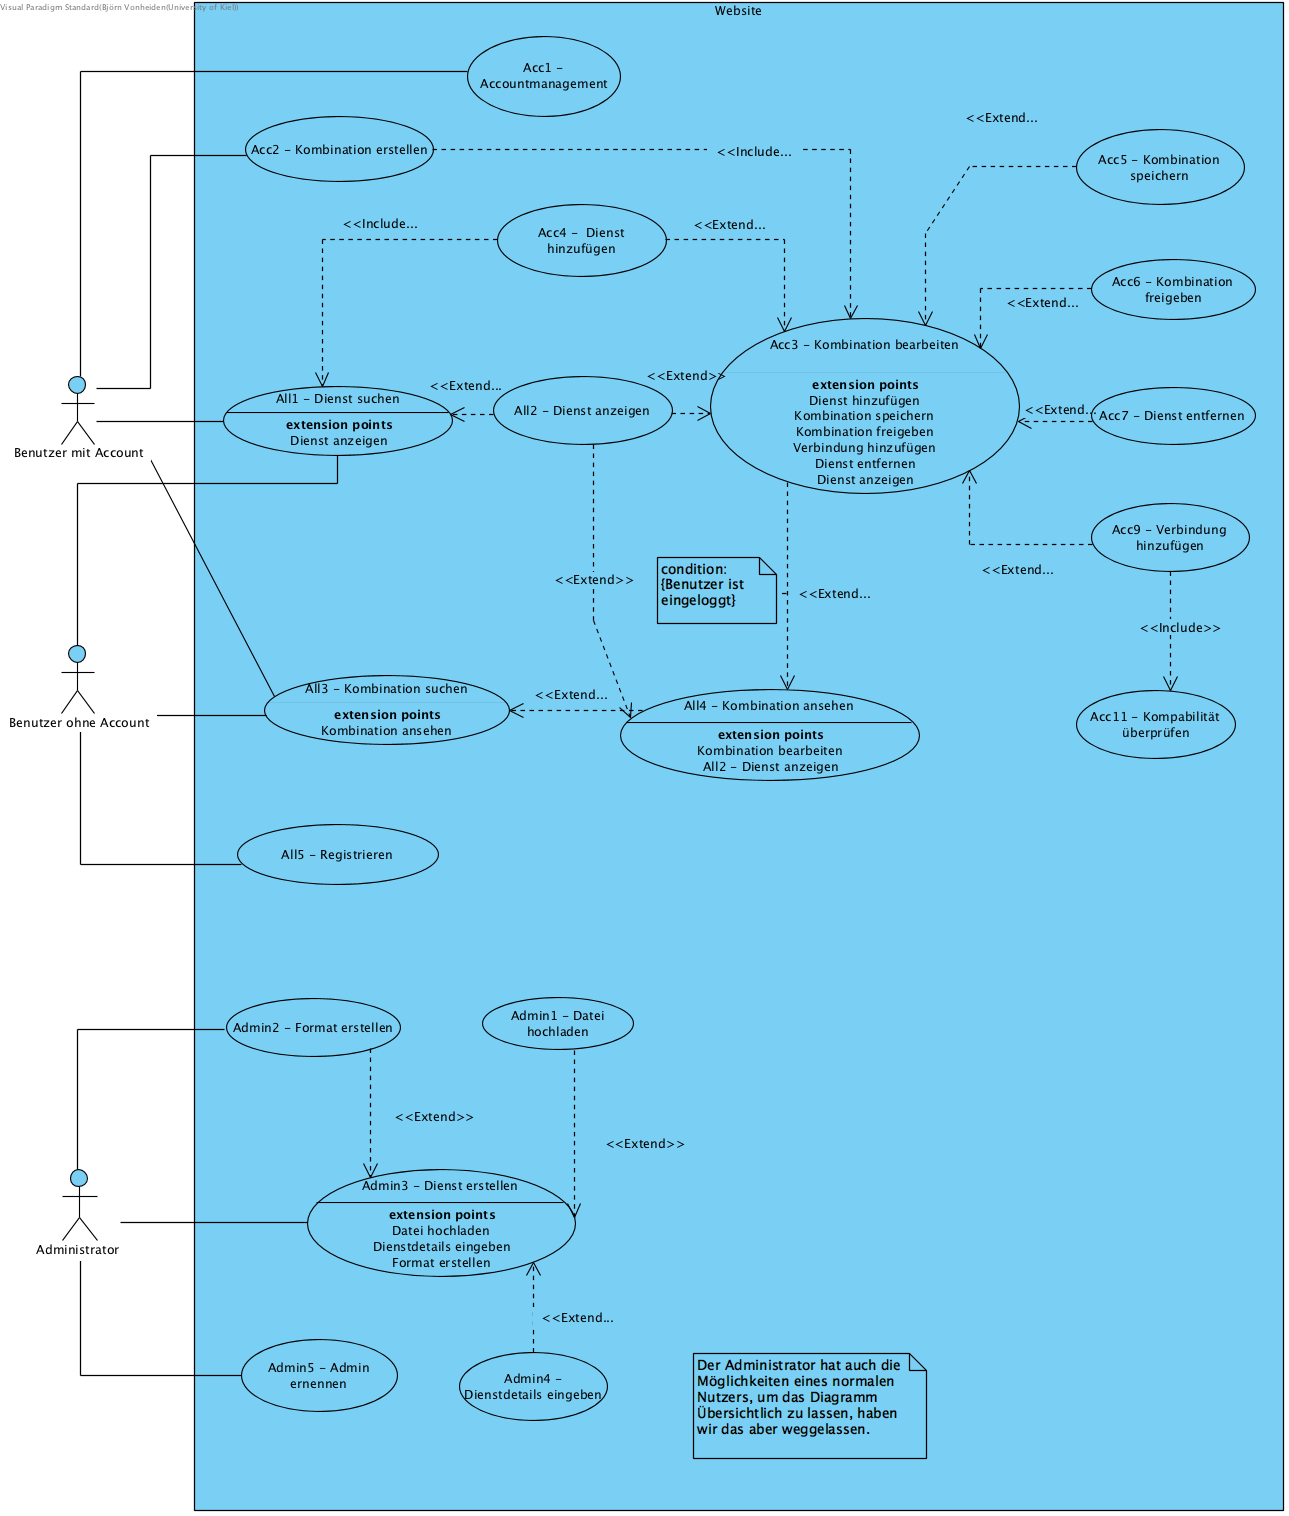
\includegraphics[width=\textwidth,height=15.5cm,keepaspectratio]{img/website}
	\caption{Anwendungsfalldiagramm - Server}
	\label{fig:anwendungsfalldiagramm-server}
\end{figure}

\newpage

\begin{figure}[h]
	\centering
	\begin{tabularx}{\textwidth}{ X | X }
		\textbf{Anwendungsfall ID} & Acc2 \\ \hline
		\textbf{Anwendungsfallname} & Kombination erstellen \\ \hline
		\textbf{Initiierender Akteur} & Benutzer mit Account / Administrator \\ \hline
		\textbf{Weitere Akteure} & -  \\ \hline
		\textbf{Kurzbeschreibung} & Erstellung einer Kombination um Kompatibilität der Dienste zu überprüfen.  \\ \hline
		\textbf{Vorbedingungen} & Der Benutzer besitzt einen Account und ist eingeloggt.  \\ \hline
		\textbf{Nachbedingungen} & -  \\ \hline
		\textbf{Ablauf} &
		\begin{enumerate}
			\item Der Nutzer möchte eine Kombination erstellen und bekommt eine leere Kombination angezeigt.
			\item {[Use-Case: Kombination bearbeiten]}
		\end{enumerate} \\ \hline
		\textbf{Alternative} &
			- \\ \hline
		\textbf{Ausnahme} &
      -  \\ \hline
		\textbf{Benutzte Anwendungsfälle} &
      \begin{itemize}
        \item Kombination bearbeiten
      \end{itemize} \\ \hline
	\end{tabularx}
	\caption{Anwendungsfall Acc2}
	\label{fig:anwendungsfall-server-tabelle-xx-1}
\end{figure}

\begin{figure}[h]
	\centering
	\begin{tabularx}{\textwidth}{ X | X }
		\textbf{Anwendungsfall ID} & Admin3 \\ \hline
		\textbf{Anwendungsfallname} & Dienst erstellen \\ \hline
		\textbf{Initiierender Akteur} & Administrator\\ \hline
		\textbf{Weitere Akteure} & -  \\ \hline
		\textbf{Kurzbeschreibung} & Ein Administrator kann entweder über eine Webschnittstelle oder über eine Datei einen neuen Dienst erstellen.  \\ \hline
		\textbf{Vorbedingungen} & Der Nutzer ist eingeloggt und besitzt Administratorrechte.  \\ \hline
		\textbf{Nachbedingungen} & Der Dienst wurde erstellt und ist jetzt von allen Nutzern sichtbar.  \\ \hline
		\textbf{Ablauf} &
		\begin{enumerate}
			\item Administrator wählt Webschnittstelle.
      \item {[Use-Case: Format erstellen]}
			\item {[Use-Case: Dienstdetails eingeben]}
			\item Der Administrator speichert den Dienst.
		\end{enumerate} \\ \hline
		\textbf{Alternative} &
    \begin{enumerate}
			\item Administrator wählt Dateischnittstelle.
			\item {[Use-Case: Datei hochladen]}
			\item Der Administrator speichert die hinzugefügten Dienste.
		\end{enumerate} \\ \hline
		\textbf{Ausnahme} &
    \begin{enumerate}
			\item Administrator wählt Webschnittstelle.
			\item {[Use-Case: Dienstdetails eingeben]}
			\item Der Administrator speichert den Dienst.
      \item Der Administrator bekommt eine Fehlermeldung, da Dienst schon vorhanden.
		\end{enumerate} \\ \hline
    \textbf{Ausnahme 2} &
		\begin{enumerate}
			\item Der Administrator wählt Datei hochladen.
			\item {[Use-Case: Datei hochladen]}
			\item Datei kann nicht gelesen werden, es gibt eine Fehlermeldung.
			\item Der Administrator kann eine neue Datei auswählen oder abbrechen.
		\end{enumerate}  \\ \hline
		\textbf{Benutzte Anwendungsfälle} &
    \begin{itemize}
			\item Datei hochladen
			\item Dienstdetails eingeben
      \item Format erstellen
		\end{itemize} \\ \hline
	\end{tabularx}
	\caption{Anwendungsfall Admin3}
	\label{fig:anwendungsfall-server-tabelle-xx-1}
\end{figure}
\begin{figure}[h]
	\centering
	\begin{tabularx}{\textwidth}{ X | X }
		\textbf{Anwendungsfall ID} & Acc3 \\ \hline
		\textbf{Anwendungsfallname} & Kombination bearbeiten \\ \hline
		\textbf{Initiierender Akteur} & Benutzer mit Account\\ \hline
		\textbf{Weitere Akteure} & -  \\ \hline
		\textbf{Kurzbeschreibung} & Ein Nutzer kann eine Kombination erstellen und bearbeiten.  \\ \hline
		\textbf{Vorbedingungen} & Der Nutzer ist eingeloggt und es gibt Kombination.  \\ \hline
		\textbf{Nachbedingungen} & -  \\ \hline
		\textbf{Ablauf} &
		\begin{enumerate}
      \item {[Use-Case: Dienst hinzufügen]} (ggf. mehrmals)
			\item {[Use-Case: Dienst entfernen]} (ggf. mehrmals)
			\item {[Use-Case: Verbindung hinzufügen]}
			\item {[Use-Case: Kombination speichern]}
			\item {[Use-Case: Kombination freigeben]}
		\end{enumerate} \\ \hline
		\textbf{Alternative} &
		\begin{enumerate}
			\item {[Use-Case: Dienst entfernen]}
			\item {[Use-Case: Kombination speichern]}
		\end{enumerate}  \\ \hline
		\textbf{Ausnahme} &
		- \\ \hline
		\textbf{Benutzte Anwendungsfälle} &
    \begin{itemize}
			\item Dienst hinzufügen
			\item Dienst entfernen
      \item Verbindung hinzufügen
      \item Kombination speichern
      \item Kombination freigeben
		\end{itemize} \\ \hline
	\end{tabularx}
	\caption{Anwendungsfall Acc3}
	\label{fig:anwendungsfall-server-tabelle-xx-1}
\end{figure}
